\documentclass{standalone}
\usepackage{tikz}
\usetikzlibrary{patterns, positioning}


\begin{document}
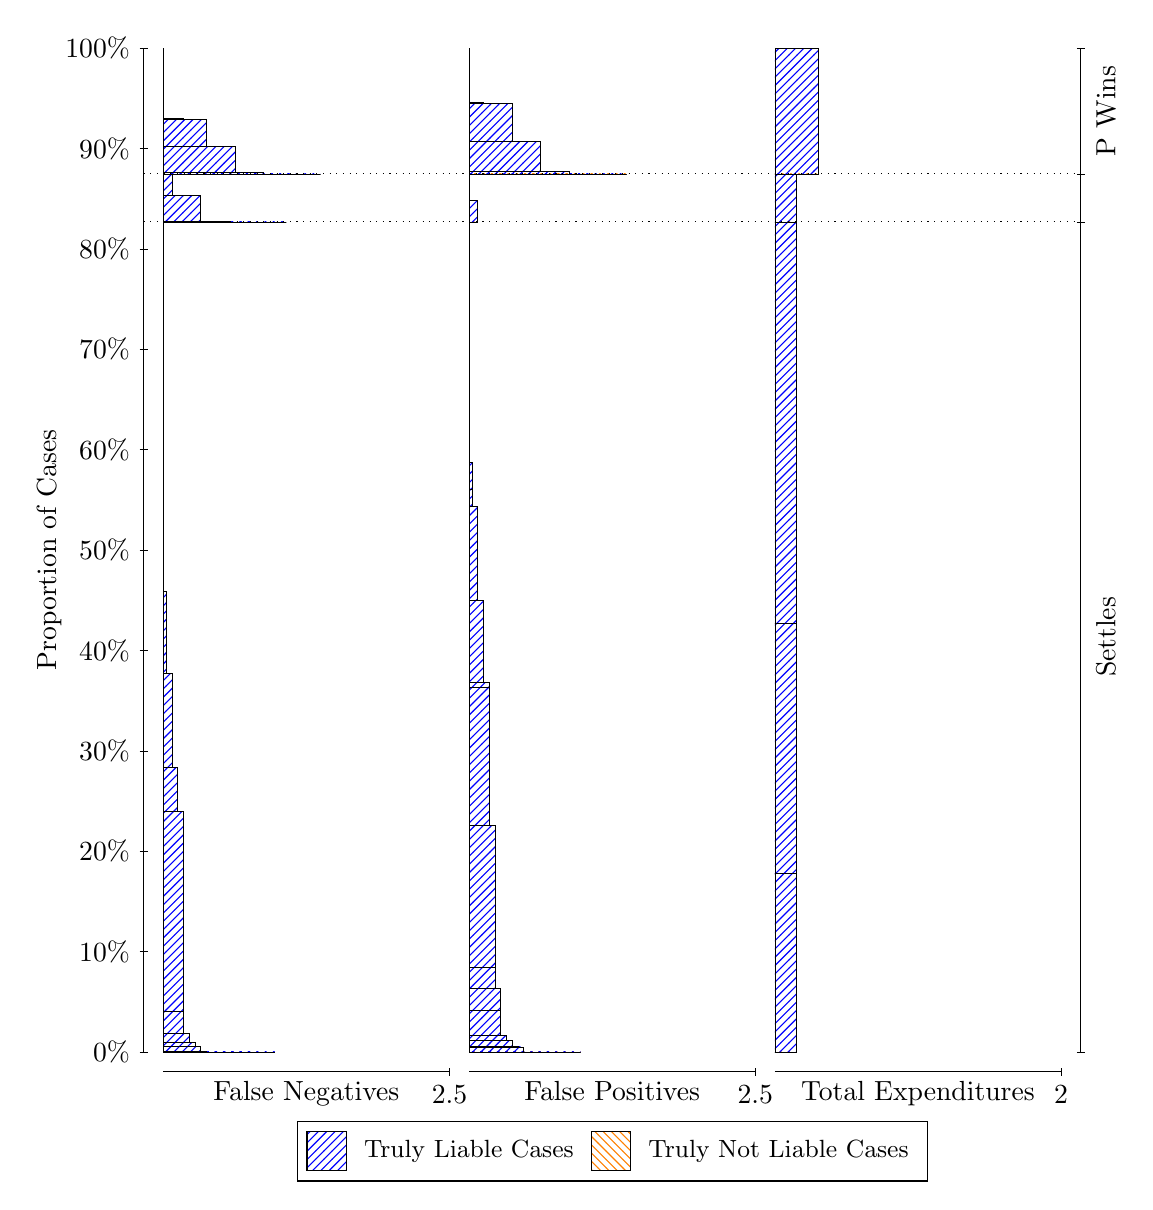
\begin{tikzpicture}
\draw[black, very thin] (1.5,1.75) -- (1.5,14.5);
\node[rotate=90, text=black, anchor=center] at (0.3, 8.125) {Proportion of Cases};
\draw[black, very thin] (1.45,1.75) -- (1.55,1.75);
\node[text=black, anchor=east] at (1.45, 1.75) {0\%};
\draw[black, very thin] (1.45,3.025) -- (1.55,3.025);
\node[text=black, anchor=east] at (1.45, 3.025) {10\%};
\draw[black, very thin] (1.45,4.3) -- (1.55,4.3);
\node[text=black, anchor=east] at (1.45, 4.3) {20\%};
\draw[black, very thin] (1.45,5.575) -- (1.55,5.575);
\node[text=black, anchor=east] at (1.45, 5.575) {30\%};
\draw[black, very thin] (1.45,6.85) -- (1.55,6.85);
\node[text=black, anchor=east] at (1.45, 6.85) {40\%};
\draw[black, very thin] (1.45,8.125) -- (1.55,8.125);
\node[text=black, anchor=east] at (1.45, 8.125) {50\%};
\draw[black, very thin] (1.45,9.4) -- (1.55,9.4);
\node[text=black, anchor=east] at (1.45, 9.4) {60\%};
\draw[black, very thin] (1.45,10.675) -- (1.55,10.675);
\node[text=black, anchor=east] at (1.45, 10.675) {70\%};
\draw[black, very thin] (1.45,11.95) -- (1.55,11.95);
\node[text=black, anchor=east] at (1.45, 11.95) {80\%};
\draw[black, very thin] (1.45,13.225) -- (1.55,13.225);
\node[text=black, anchor=east] at (1.45, 13.225) {90\%};
\draw[black, very thin] (1.45,14.5) -- (1.55,14.5);
\node[text=black, anchor=east] at (1.45, 14.5) {100\%};

\draw[black, very thin] (13.4,1.75) -- (13.4,14.5);
\draw[black, very thin] (13.35,1.75) -- (13.45,1.75);
\node[anchor=west] at (13.35, 1.75) {};
\draw[black, very thin] (13.35,12.292) -- (13.45,12.292);
\node[anchor=west] at (13.35, 12.292) {};
\draw[black, very thin] (13.35,12.902) -- (13.45,12.902);
\node[anchor=west] at (13.35, 12.902) {};
\draw[black, very thin] (13.35,14.5) -- (13.45,14.5);
\node[anchor=west] at (13.35, 14.5) {};

\draw[black, very thin, pattern color=blue, pattern=north east lines] (1.75,1.75) rectangle (3.167,1.75);
\draw[black, very thin, pattern color=blue, pattern=north east lines] (1.75,1.75) rectangle (3.0217,1.75);
\draw[black, very thin, pattern color=blue, pattern=north east lines] (1.75,1.75) rectangle (2.8763,1.75);
\draw[black, very thin, pattern color=blue, pattern=north east lines] (1.75,1.75) rectangle (2.8037,1.75);
\draw[black, very thin, pattern color=blue, pattern=north east lines] (1.75,1.75) rectangle (2.731,1.75);
\draw[black, very thin, pattern color=blue, pattern=north east lines] (1.75,1.75) rectangle (2.6583,1.75);
\draw[black, very thin, pattern color=blue, pattern=north east lines] (1.75,1.75) rectangle (2.5857,1.75);
\draw[black, very thin, pattern color=blue, pattern=north east lines] (1.75,1.75) rectangle (2.513,1.75);
\draw[black, very thin, pattern color=blue, pattern=north east lines] (1.75,1.75) rectangle (2.4403,1.7501);
\draw[black, very thin, pattern color=blue, pattern=north east lines] (1.75,1.7501) rectangle (2.3677,1.7507);
\draw[black, very thin, pattern color=blue, pattern=north east lines] (1.75,1.7507) rectangle (2.295,1.7552);
\draw[black, very thin, pattern color=blue, pattern=north east lines] (1.75,1.7552) rectangle (2.2223,1.8185);
\draw[black, very thin, pattern color=blue, pattern=north east lines] (1.75,1.8185) rectangle (2.1497,1.8727);
\draw[black, very thin, pattern color=blue, pattern=north east lines] (1.75,1.8727) rectangle (2.077,1.9876);
\draw[black, very thin, pattern color=blue, pattern=north east lines] (1.75,1.9876) rectangle (2.0043,2.2614);
\draw[black, very thin, pattern color=blue, pattern=north east lines] (1.75,2.2614) rectangle (2.0043,4.8032);
\draw[black, very thin, pattern color=blue, pattern=north east lines] (1.75,4.8032) rectangle (1.9317,5.3669);
\draw[black, very thin, pattern color=blue, pattern=north east lines] (1.75,5.3669) rectangle (1.859,6.556);
\draw[black, very thin, pattern color=blue, pattern=north east lines] (1.75,6.556) rectangle (1.7863,7.5997);
\draw[black, very thin, pattern color=orange, pattern=north west lines] (1.75,7.5997) rectangle (1.75,7.5997);
\draw[black, very thin, pattern color=blue, pattern=north east lines] (1.75,7.5997) rectangle (1.75,12.292);
\draw[black, very thin, pattern color=blue, pattern=north east lines] (1.75,12.292) rectangle (3.3123,12.292);
\draw[black, very thin, pattern color=blue, pattern=north east lines] (1.75,12.292) rectangle (2.949,12.292);
\draw[black, very thin, pattern color=blue, pattern=north east lines] (1.75,12.292) rectangle (2.5857,12.3);
\draw[black, very thin, pattern color=blue, pattern=north east lines] (1.75,12.3) rectangle (2.2223,12.629);
\draw[black, very thin, pattern color=blue, pattern=north east lines] (1.75,12.629) rectangle (1.859,12.902);
\draw[black, very thin, pattern color=orange, pattern=north west lines] (1.75,12.902) rectangle (1.75,12.902);
\draw[black, very thin, pattern color=blue, pattern=north east lines] (1.75,12.902) rectangle (3.7483,12.902);
\draw[black, very thin, pattern color=blue, pattern=north east lines] (1.75,12.902) rectangle (3.385,12.902);
\draw[black, very thin, pattern color=blue, pattern=north east lines] (1.75,12.902) rectangle (3.0217,12.924);
\draw[black, very thin, pattern color=blue, pattern=north east lines] (1.75,12.924) rectangle (2.731,12.924);
\draw[black, very thin, pattern color=blue, pattern=north east lines] (1.75,12.924) rectangle (2.6583,13.248);
\draw[black, very thin, pattern color=blue, pattern=north east lines] (1.75,13.248) rectangle (2.3677,13.248);
\draw[black, very thin, pattern color=blue, pattern=north east lines] (1.75,13.248) rectangle (2.295,13.589);
\draw[black, very thin, pattern color=blue, pattern=north east lines] (1.75,13.589) rectangle (2.0043,13.606);
\draw[black, very thin, pattern color=blue, pattern=north east lines] (1.75,13.606) rectangle (1.9317,13.607);
\draw[black, very thin, pattern color=orange, pattern=north west lines] (1.75,13.607) rectangle (1.75,13.607);
\draw[black, very thin, pattern color=blue, pattern=north east lines] (1.75,13.607) rectangle (1.75,14.5);
\draw[black, very thin, pattern color=orange, pattern=north west lines] (5.6333,1.75) rectangle (7.0503,1.75);
\draw[black, very thin, pattern color=blue, pattern=north east lines] (5.6333,1.75) rectangle (7.0503,1.75);
\draw[black, very thin, pattern color=orange, pattern=north west lines] (5.6333,1.75) rectangle (6.7597,1.75);
\draw[black, very thin, pattern color=blue, pattern=north east lines] (5.6333,1.75) rectangle (6.7597,1.75);
\draw[black, very thin, pattern color=blue, pattern=north east lines] (5.6333,1.75) rectangle (6.687,1.75);
\draw[black, very thin, pattern color=orange, pattern=north west lines] (5.6333,1.75) rectangle (6.6143,1.75);
\draw[black, very thin, pattern color=blue, pattern=north east lines] (5.6333,1.75) rectangle (6.6143,1.75);
\draw[black, very thin, pattern color=orange, pattern=north west lines] (5.6333,1.75) rectangle (6.469,1.75);
\draw[black, very thin, pattern color=blue, pattern=north east lines] (5.6333,1.75) rectangle (6.469,1.75);
\draw[black, very thin, pattern color=blue, pattern=north east lines] (5.6333,1.75) rectangle (6.3963,1.7506);
\draw[black, very thin, pattern color=orange, pattern=north west lines] (5.6333,1.7506) rectangle (6.3237,1.7506);
\draw[black, very thin, pattern color=blue, pattern=north east lines] (5.6333,1.7506) rectangle (6.3237,1.7513);
\draw[black, very thin, pattern color=blue, pattern=north east lines] (5.6333,1.7513) rectangle (6.3237,1.8155);
\draw[black, very thin, pattern color=blue, pattern=north east lines] (5.6333,1.8155) rectangle (6.251,1.8179);
\draw[black, very thin, pattern color=orange, pattern=north west lines] (5.6333,1.8179) rectangle (6.1783,1.8179);
\draw[black, very thin, pattern color=blue, pattern=north east lines] (5.6333,1.8179) rectangle (6.1783,1.8945);
\draw[black, very thin, pattern color=blue, pattern=north east lines] (5.6333,1.8945) rectangle (6.1057,1.9583);
\draw[black, very thin, pattern color=orange, pattern=north west lines] (5.6333,1.9583) rectangle (6.033,1.9583);
\draw[black, very thin, pattern color=blue, pattern=north east lines] (5.6333,1.9583) rectangle (6.033,2.2766);
\draw[black, very thin, pattern color=blue, pattern=north east lines] (5.6333,2.2766) rectangle (6.033,2.5528);
\draw[black, very thin, pattern color=blue, pattern=north east lines] (5.6333,2.5528) rectangle (5.9603,2.8274);
\draw[black, very thin, pattern color=blue, pattern=north east lines] (5.6333,2.8274) rectangle (5.9603,4.6315);
\draw[black, very thin, pattern color=orange, pattern=north west lines] (5.6333,4.6315) rectangle (5.8877,4.6315);
\draw[black, very thin, pattern color=blue, pattern=north east lines] (5.6333,4.6315) rectangle (5.8877,6.3791);
\draw[black, very thin, pattern color=blue, pattern=north east lines] (5.6333,6.3791) rectangle (5.8877,6.4427);
\draw[black, very thin, pattern color=blue, pattern=north east lines] (5.6333,6.4427) rectangle (5.815,7.4865);
\draw[black, very thin, pattern color=blue, pattern=north east lines] (5.6333,7.4865) rectangle (5.7423,8.6755);
\draw[black, very thin, pattern color=blue, pattern=north east lines] (5.6333,8.6755) rectangle (5.6697,8.9014);
\draw[black, very thin, pattern color=blue, pattern=north east lines] (5.6333,8.9014) rectangle (5.6697,9.2393);
\draw[black, very thin, pattern color=blue, pattern=north east lines] (5.6333,9.2393) rectangle (5.6333,12.292);
\draw[black, very thin, pattern color=orange, pattern=north west lines] (5.6333,12.292) rectangle (5.7423,12.292);
\draw[black, very thin, pattern color=blue, pattern=north east lines] (5.6333,12.292) rectangle (5.7423,12.565);
\draw[black, very thin, pattern color=blue, pattern=north east lines] (5.6333,12.565) rectangle (5.6333,12.902);
\draw[black, very thin, pattern color=orange, pattern=north west lines] (5.6333,12.902) rectangle (7.6317,12.902);
\draw[black, very thin, pattern color=blue, pattern=north east lines] (5.6333,12.902) rectangle (7.6317,12.902);
\draw[black, very thin, pattern color=orange, pattern=north west lines] (5.6333,12.902) rectangle (7.2683,12.902);
\draw[black, very thin, pattern color=blue, pattern=north east lines] (5.6333,12.902) rectangle (7.2683,12.902);
\draw[black, very thin, pattern color=orange, pattern=north west lines] (5.6333,12.902) rectangle (6.905,12.902);
\draw[black, very thin, pattern color=blue, pattern=north east lines] (5.6333,12.902) rectangle (6.905,12.931);
\draw[black, very thin, pattern color=orange, pattern=north west lines] (5.6333,12.931) rectangle (6.5417,12.931);
\draw[black, very thin, pattern color=blue, pattern=north east lines] (5.6333,12.931) rectangle (6.5417,13.312);
\draw[black, very thin, pattern color=orange, pattern=north west lines] (5.6333,13.312) rectangle (6.251,13.312);
\draw[black, very thin, pattern color=blue, pattern=north east lines] (5.6333,13.312) rectangle (6.251,13.312);
\draw[black, very thin, pattern color=blue, pattern=north east lines] (5.6333,13.312) rectangle (6.1783,13.795);
\draw[black, very thin, pattern color=blue, pattern=north east lines] (5.6333,13.795) rectangle (5.8877,13.795);
\draw[black, very thin, pattern color=orange, pattern=north west lines] (5.6333,13.795) rectangle (5.8877,13.795);
\draw[black, very thin, pattern color=blue, pattern=north east lines] (5.6333,13.795) rectangle (5.8877,13.795);
\draw[black, very thin, pattern color=blue, pattern=north east lines] (5.6333,13.795) rectangle (5.815,13.813);
\draw[black, very thin, pattern color=orange, pattern=north west lines] (5.6333,13.813) rectangle (5.6333,13.813);
\draw[black, very thin, pattern color=blue, pattern=north east lines] (5.6333,13.813) rectangle (5.6333,14.5);
\draw[black, very thin, pattern color=orange, pattern=north west lines] (9.5167,1.75) rectangle (9.7892,1.75);
\draw[black, very thin, pattern color=blue, pattern=north east lines] (9.5167,1.75) rectangle (9.7892,4.0191);
\draw[black, very thin, pattern color=orange, pattern=north west lines] (9.5167,4.0191) rectangle (9.7892,4.0191);
\draw[black, very thin, pattern color=blue, pattern=north east lines] (9.5167,4.0191) rectangle (9.7892,7.1948);
\draw[black, very thin, pattern color=orange, pattern=north west lines] (9.5167,7.1948) rectangle (9.7892,7.1948);
\draw[black, very thin, pattern color=blue, pattern=north east lines] (9.5167,7.1948) rectangle (9.7892,12.292);
\draw[black, very thin, pattern color=orange, pattern=north west lines] (9.5167,12.292) rectangle (9.7892,12.292);
\draw[black, very thin, pattern color=blue, pattern=north east lines] (9.5167,12.292) rectangle (9.7892,12.902);
\draw[black, very thin, pattern color=orange, pattern=north west lines] (9.5167,12.902) rectangle (10.062,12.902);
\draw[black, very thin, pattern color=blue, pattern=north east lines] (9.5167,12.902) rectangle (10.062,14.5);
\draw[black, dotted] (1.5,12.292) -- (13.4,12.292);
\draw[black, dotted] (1.5,12.902) -- (13.4,12.902);
\draw[black, very thin] (1.75,1.5) -- (5.3833,1.5);
\node[text=black, anchor=north] at (3.5667, 1.5) {False Negatives};
\draw[black, very thin] (5.3833,1.45) -- (5.3833,1.55);
\node[text=black, anchor=north] at (5.3833, 1.45) {2.5};

\draw[black, very thin] (5.6333,1.5) -- (9.2667,1.5);
\node[text=black, anchor=north] at (7.45, 1.5) {False Positives};
\draw[black, very thin] (9.2667,1.45) -- (9.2667,1.55);
\node[text=black, anchor=north] at (9.2667, 1.45) {2.5};

\draw[black, very thin] (9.5167,1.5) -- (13.15,1.5);
\node[text=black, anchor=north] at (11.333, 1.5) {Total Expenditures};
\draw[black, very thin] (13.15,1.45) -- (13.15,1.55);
\node[text=black, anchor=north] at (13.15, 1.45) {2};

\node[text=black, centered, rotate=90] at (13.72, 7.0212) {Settles};

\node[text=black, centered, rotate=90] at (13.72, 13.701) {P Wins};

\draw (7.449999999999999,1.5) node[draw=none] (baseCoordinate) {};
\begin{scope}[align=center]
        \matrix[scale=0.5, draw=black, below=0.5cm of baseCoordinate, nodes={draw}, column sep=0.1cm]{
            \node[rectangle, draw, minimum width=0.5cm, minimum height=0.5cm, pattern color=blue, pattern=north east lines] {}; &
            \node[draw=none, font=\small, text=black] (B) {Truly Liable Cases}; &
            \node[rectangle, draw, minimum width=0.5cm, minimum height=0.5cm, pattern color=orange, pattern=north west lines] {}; &
            \node[draw=none, font=\small, text=black] (B) {Truly Not Liable Cases}; \\
            };
\end{scope}

\end{tikzpicture}
\end{document}